%
% Body text font is Palatino!
%

\documentclass[a5paper,pagesize,10pt,bibtotoc,pointlessnumbers,
normalheadings,DIV=9,twoside=false]{scrbook}

% twoside, openright
\KOMAoptions{DIV=last}

\usepackage{trajan}
 
\usepackage[english]{babel}
\usepackage[utf8]{inputenc}
\usepackage[T1]{fontenc}
\usepackage[table, svgnames, dvipsnames]{xcolor}
\usepackage{makecell, cellspace, caption}

\usepackage{graphicx}
\graphicspath{ {./graphics/} }

\usepackage[babel,german=guillemets]{csquotes}

\usepackage[sc]{mathpazo}
\linespread{1.05} 

\usepackage{verbatim} % for comments
\usepackage{listings} % for comments

%\setlength{\parindent}{10pt}
%\setlength{\parskip}{1.4ex plus 0.35ex minus 0.3ex}
%\setlength{\parskip}{1.4ex plus 0.35ex minus 0.3ex}

\usepackage{blindtext}
\newcommand{\q}[1]{>>\textit{#1}<<}

\newcommand{\cardbuilding}[8]
{
	 \hline
	  \rowcolor{Gainsboro!60}
	#1 & #2 Gold  \\
	\hline
	Lifepoints & #7 \\
	Defense & #8 \\
%	\hline
	Upgradeslots & #3  \\
%	Upgradeslot 1 & #3  \\
%	Upgradeslot 2 & #4 \\
%	Upgradeslot 3 & #5 \\
	\hline
	 \multicolumn{2}{||l||}{\parbox{14cm}{\textbf{Ruletext:} #6}}\\
	\hline
}

\newcommand{\card}[2]
{
	 \hline
	#1 & #2  \\
	\hline
}




\title{A Game of Micro and Macro}   
\author{Robert Zeßin} 
\date{\today} 

\begin{document}

\begin{titlepage}
		\centering{
			{\fontsize{40}{48}\selectfont 
			A Game of Micro and Macro}
		}\\
			
		\vspace{10mm}
		\centering{\Large{Robert Zeßin}}\\
		\vspace{\fill}
		\centering \large{2021}
\end{titlepage}

\newpage
\chapter{Intro}

A Game of Micro and Macro is a two-player boardgame consisting of two parts.

A tabletop-style skirmish game, in which units battle against each other and a card-laying game in which both players build a base to support their units on the battlefields.

The rules and materials nessecary to play this game are descriped in this book.

\newpage
\tableofcontents 


\newpage
\chapter{General Rules}

\section{Preparation}
Before the game starts some preparations have to be made for both parts of the game.

The first action is to check who gets priority. For that matter both players roll a D6. The player with the highes value gets the first priority. Reroll on a tie.

\subsection{Micro}
The battlefield is build up. Each player picks an even amount of terrain-pices. Both players place their pices alternating on the board.

The miniatures (models/units) used during the game a placed next to the board.

Both players teach each other about their units. This does not have to include possible modifications to the units made during the macro-game.

Both players place a marker on the board representing the entrypoint of the macrogame.

\subsection{Macro}
Both players shuffle their decks and place them face down to the side. Buildingcards a placed in the bottom. Right in front of them is their mainbuilding card. Each player draws five cards from their deck.

To keep track of game stats like the amount of available ressources and lifepoints a fair amount of spindown-dice or pen and paper are in reach.

\begin{figure}[t]
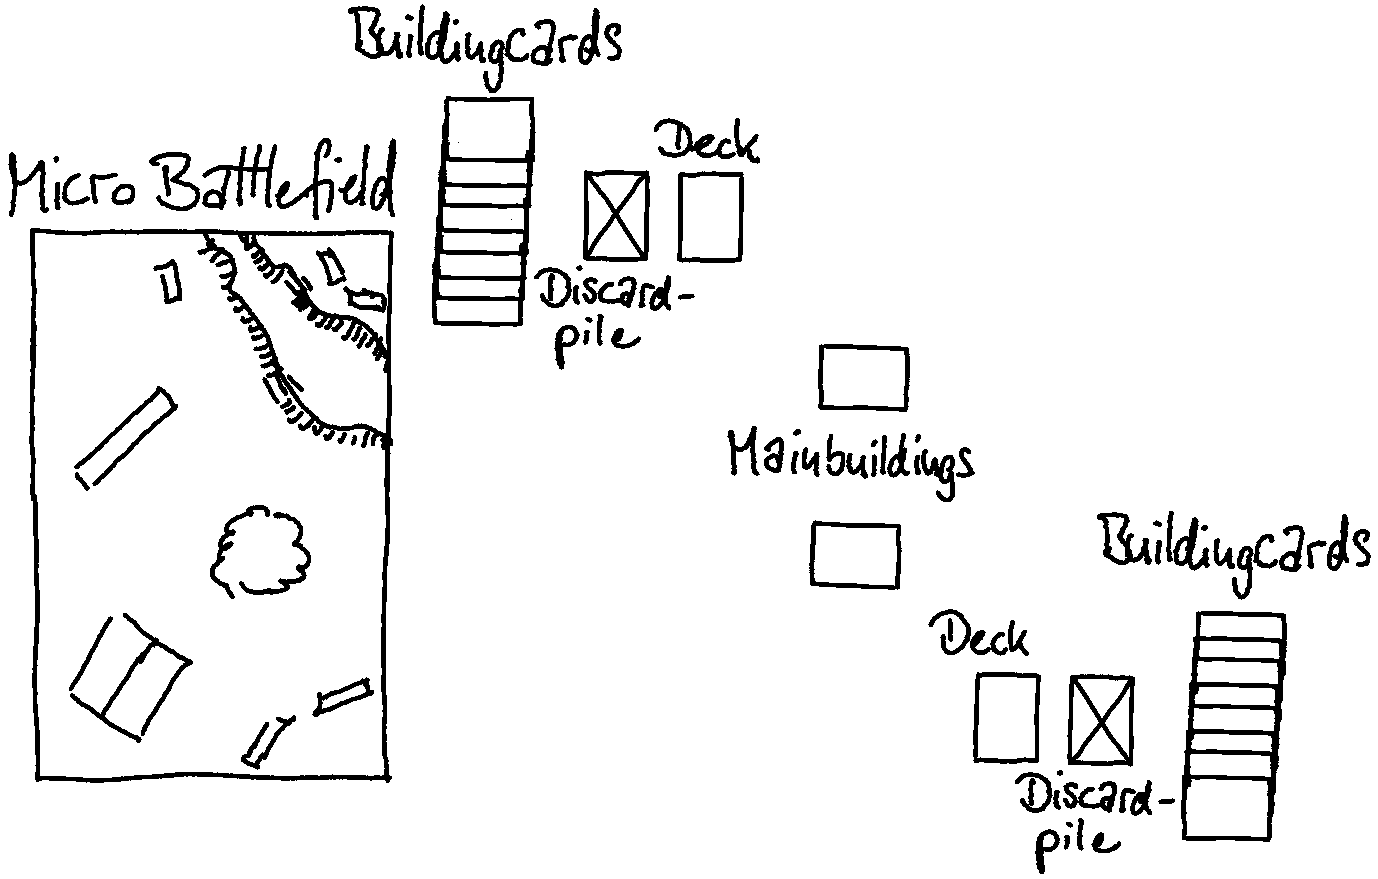
\includegraphics[scale=0.25]{Boardoverview}
\centering
\caption{Overview of a fresh game}
\end{figure}

\section{A turn}
A turn is structured as follows.

\begin{enumerate}
\item the player with priority draws one cards
\item triggered abilities of buildings and upgrades are played
\item the player with priority takes three actions from the following list
\begin{enumerate}
\item command a unit in the micro-game
\item build a unit from a building or upgrade
\item use a card-ability
\item play a card from his hand
\item pass the turn
\end{enumerate}
\end{enumerate}

After each action, the other player has the opportunity to react. As a reaction cards with the attribute \emph{instant} can be played.\\
\\
After each action, or reaction it is checked if the game is finished.\\
\\
If all actions are made, priority changes and the next turn starts.

\section{End of Game}
A game is finished if the main-building of a player is destroyed. This player has lost the game.\\
\\
A game is also finished if a player is not able to perform an action other then passing the turn. This player has lost the game.\\
\\
Other then that, a player is alowed to concede at any time.


\section{Out of Cards}
If a player is out of cards to draw from his deck his main-building is dealt one damage. This is done for each card.
If a player needs to draw two cards, the mailbuildung is dealt two damage.\\


\section{Base-range}
Baserange descripes the radius of a base starting from the center of the base-marker. The radius changes with the number of building inside the base.
The range of the base is always checked if the number of buildings change or another action needs to know the current radius.

The range of the base is set as follows

\begin{center}
 \begin{tabular}{||c c||} 
 \hline
 No. of Buildings & Radius\\
 \hline\hline
 1 & 1 \\ 
 \hline
 2 & 1.5 \\
 \hline
 3 & 2 \\
 \hline
 4 & 2.5\\
 \hline
 5 & .. \\
 \hline
\end{tabular}
\end{center}

The base range is needed for attack made by units against the base.


\chapter{Micro}

Micro is a skirmish miniature game. Each player has a set of miniature which can come into play.

Each Miniature, or type of miniature has a fixed set of attributes and skills which makes them unique.

\section{Attributes}
Each attribute, except for movement and lifepoints, is represented by a dice. The amount of surfaces indicates how powerfull the attribute is.
That does not mean that you need a die for each attribute of each model. One set of dice will do.

Surface count goes from 4 (D4) - weak, to 20 (D20) - strong. In between are D6, 8, 10, 12 and 16.

If something causes an attribute to increase by an amount, it means ti increase the die used. For example if a unit has an attack of D4. an increase by two ups it to D8.\\
\\
Movement and Lifepoints are plain values between 1 and 100

\begin{description}
\item[Lifepoints (LP)]
Amount of damage nessecary to kill a unit
\item[Movement (M)]
maximum amount a unit can move in centimeters
\item[Attack (A)]
Strength of a physical attack
\item[Spellpower (SP)]
Strength of a magical attack
\item[Defence (D)]
Ability to withstand a physical attack
\item[Magic Defence (MD)]
Ability to withstand a magical attack
\end{description}

\section{Roll-Off}
In a Roll-Off both players roll a die. The attacker wins if is value is greater the the value of the defender.

If a die rolls its highes possible score, the player can add seven to the value. This counts as a crit and enables smaller units to hit a big blow against bigger foes.

\section{Allocating Damage}
To deal damage from one unit to another the corresponding attributes of attacker and defender clash in a roll off.

For physical damage (A) and (D) are taken to a roll off. For a magic attack (SP) and (MD).

If the attack is physical or magic is the choice of the attacker, but is determined by some factores like range, visibility and the kind of items a unit has.\\
\\
For example, if a unit is equiped with a rusty sword and knows the leech seed spell its options is to do a meele-attack with its rusty sword, if a unit is nearby, or hurl its leech seed onto a target which is within the range of the spell and can be seen by the unit.\\
To see a unit, virtualy draw a line between the attacker and target. This line should not be interupted by any kind of terrain.

\section{Micro-Actions}
If a player decides to command a unit as one of his two game-actions he has the following options.

\begin{enumerate}
\item Pick a unit or unit-group
\item Pick a unit-action and use it
\item Pick another, or the same unit-action and use it
\end{enumerate}

\subsection{Unit-Group}
Units of the same kind ,or bound through other rules, with a maxium distance of two to each other can be commanded as a group.

\subsection{Unit-Action}
Units have the following actions.

\begin{enumerate}
\item Moving
\item Physical Attack
\item Magical Attack
\item Entrench/Mobilize
\end{enumerate}

\subsubsection{Moving}
The unit or group moves its maximum movement-value, or less.
In a group, each unit uses its own movement-value. Single units of a group may loose the connection to the group. These units do not participade in other actions done by the group.

\subsubsection{Physical Attack}
To make a physical attack a unit, or group, uses its equiped weapon, or weapon set. 
A unit can only carry one weapon, or weapon set.
What weapon or weapon set is carried is determined by the building which produced the unit. The wilded weapon can be changed with upgrade-cards in the macro-game.
All units start with a weapon or basic attack-effekt.\\
\\
Each weapon has a range in which the target has to be. Meele-weapons, e.g. Swords, have a range of one.\\
\\
Weapons can have extra effekts. These can be triggered on a attack or permanent effects on the carrier and its stats.\\
%\\
%All weapons can be carried by all units, if no effekt says otherwise.\\
%\\
%If a Unit dies a attacker in meele-range can pick up the defenders weapon and use it.

\subsubsection{Magical Attack}
To make a magical attack a unit needs to be able to cast a spell. Spells are learnt through playing upgradecards on buildings in the macro-game.\\
\\
Spells, like weapons, have a maximum range in which the target has to be.\\
\\
All spells have an effekt triggered after a successfull roll off. Some spells may have effekts triggered by a lost roll off.\\
\\
There are some general spells useable by all units. Most of them are special to a small number of units. Those spells are accordingly marked an ther upgrade-card. Either with the name of the unit or with the symbole of the faction/race which can use the spell.\\
\\
A Spell targeting a friendly unit does not need a roll off\\
\\
Within a group, only one unit can cast a spell.

\subsubsection{Entrench/Mobilize}
A unit, or group, can entrench themself, or mobilize if it is already entrenched.
Entrenched units, or groups, can make an attack if an enemy unit, or group, get in its attack-range.
The attack is made immediately, before any other attacks or actions.\\
After the attack, the unit, or group, is mobilized.\\
\\
Entrenched units can note make normal moves, they first have to mobilize.

\chapter{Macro}
Macro is a card-laying game in which each players builds a base. The base is then used to build and upgrade units which are send out in the micro-game to destroy the enemy base.

For that matter, each player has a custom deck of cards. A deck is made up of cards of different types.

All cards have a faction- or race-symbol. A deck can only contain cards of the same symbol. Unless a rule says otherwise.

\section{Cardtypes}
Cardtypes determine where and who a card is played. The following cardtypes exist.

\begin{enumerate}
\item Buildings
\item Upgrades
\item Instants
\end{enumerate}

\subsection{Buildings}
Buildings are factiondependant and marked with the factions symbol. Each Building as a number of lifepoints and a defence-attribute.
Units can deal damage to buildings and reduce the points. If a building has no lifepoints left it is destroyed.\\
\\
A Building usualy has a ruletext which includes active abilities or triggered cardeffects.\\
\\
A Building has upgradeslots, up to a maximum of three.
Upgradecards can be played onto building. Some upgrades require to be played on special buildings or have other conditions.

\begin{figure}[t]
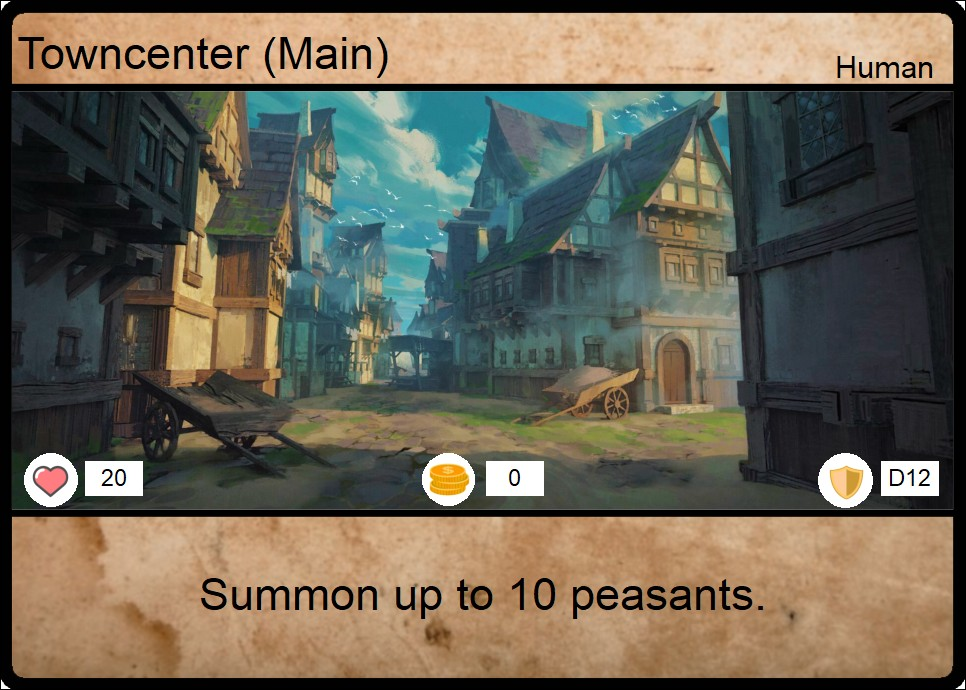
\includegraphics[scale=1.0]{examplebuilding}
\centering
\caption{Anatomy of a building}
\end{figure}

\subsubsection{Build buildings}
To build a building a buildingcard is selected from the pile of buildingcards next to the playingfield. Its ressource-costs need to be paid as it enters the battlefield.
New buildings a place to the left side of the last placed building.

\subsubsection{Dealing damage to buildings}
Damage to buildings is dealt by units from the micro-game. The same rules to a roll-off apply. If a unit is in range to the base-marker of an enemy-base it attacks the most left building.\\
\\
To deal damage to the base, or buildings, a unit needs to be in attack-range. This includes the range of its own weapon and the radius the base has, determined by the number of buildings in it.

\subsection{Upgrades}
Upgrades are cards played onto buildings. Upgrades modify units and/or the buildings they are played on. Some upgrade can only be played on certain building or have other conditions.

If an Upgradeslot is already used, it can be overwriten with a new upgrade.The upgrade which is overwritten has no effekt, unless another rule says otherwise.\\

\begin{figure}[t]
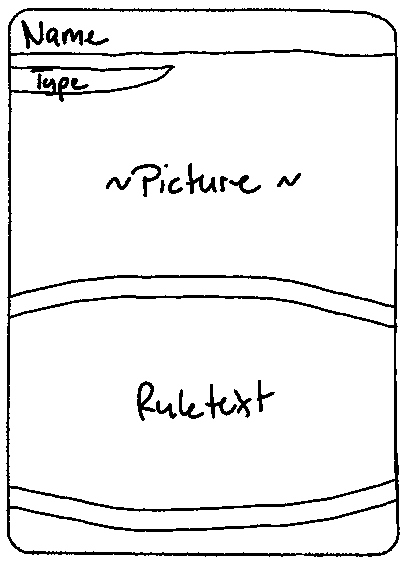
\includegraphics[scale=0.5]{Maindeckcard}
\centering
\caption{Anatomy of a maindeck-card}
\end{figure}

\subsection{Instants}
Instants a one-time effekts with an effekt which is handelt directly after it is played. Instants can be played in a players turn and in the enemys turn as a reaction to an action.\\

\newpage
\section{Cardeffects and -abilities}
Cardeffects, unless they are triggered from another event, can be activated by a player as one of their actions. A cardeffect can only be actived once per turn, unless a rules says otherwise.\\
\\
Triggered abilities are resolved emedetly they are triggered.\\
\\
Active cardeffects may have a cost which has to be payed before the effect is resolved.

\chapter{Factions and Races}
Each player has choosen a faction with which he plays a game. The choosen faction is represented by the players deck of cards, buildings and units. Each of these are kind of unique to each faction and represent a different playstyle.

In this chapter, the characteristics and units of each faction is descriped.
\newpage
\section{Kingdoms of Men}

\subsubsection{Description}
The Kingdoms of Men constits of many smaller kingdoms, loosely united by the high king. In times of need the high king commands all kingdoms under his banner.\\
In a world full of inexplicable dangers humans survive due to their adaptability. Driven by their fate they seem to achive everything.\\
\\
In times of overall peace it is not unusual for the smaller kings to feud over the favor of the high king.

\subsubsection{Keywords}
\emph{mortal, many, ambitious, resilient, principled, hierachy}

\subsubsection{Units}
 \begin{tabular}{||c c c c c c c||} 
 \hline
  & M & LP & A & D & SP & MD \\
 \hline\hline
 Peassant & 4 & 5 & D6 & D4 & D4 & D4 \\ 
  & \multicolumn{6}{l||}{\textbf{Weapon:} Rusty sword} \\
  & \multicolumn{6}{l||}{\textbf{Spells:} Mobstrength} \\
 \hline
  Townguard & 4 & 8 & D6 & D6 & D4 & D4 \\ 
  & \multicolumn{6}{l||}{\textbf{Weapon:} Sword and Board} \\
 \hline
 Knight & 6  & 12 & D8 & D10 & D6 & D8 \\
  & \multicolumn{6}{l||}{\textbf{Weapon:} Sword and Board} \\
  & \multicolumn{6}{l||}{\textbf{Spells:} Commanding presence} \\
  \hline

\end{tabular}

\newpage
\section{Bloodmages}

\subsubsection{Description}
Bloodmages are mages who have choosen a very dark path. With no way of return they are dedicated to a magic with strong bonds to the underworld.
From sacrifices and their blood the summon destructive magic only aimed for their own advantage.\\
\\
A bloodmage usualy is on its own, accompanied by demonic creatures, skeleton and zombies. As the sole backbone of this faction, a bloodmage is not reluctant to sacrifice its own allies to stay alive.

\subsubsection{Keywords}
\emph{daemonic, vicious, inconsiderate, selfdestructive}

\subsubsection{Units}
 \begin{tabular}{||c c c c c c c||} 
 \hline
  & M & LP & A & D & SP & MD \\
 \hline\hline
 Bloodmage & 5 & 20 & D6 & D6 & D16 & D12 \\ 
  & \multicolumn{6}{l||}{\textbf{Weapon:} Wooden Staff} \\
  & \multicolumn{6}{l||}{\textbf{Spells:} Demonic Leech} \\
 \hline
 Skeleton & 3 & 7 & D4 & D6 & D4 & D6 \\
  & \multicolumn{6}{l||}{\textbf{Weapon:} Rusty Sword} \\
  & \multicolumn{6}{l||}{\textbf{Spells:} Masters Presence} \\
\hline
 Direwolf & 8 & 8 & D10 & D6 & D4 & D4 \\
  & \multicolumn{6}{l||}{\textbf{Weapon:} Teeth} \\
  & \multicolumn{6}{l||}{\textbf{Spells:} Infectious bite} \\
\hline
\end{tabular}

\newpage
\section{Swampbeasts}

\subsubsection{Description}
The creatures of the swamps around the human towns and villiages in the marshes seem to have a collective mind.\\
Merchants tell stories about coordinated attacks against their tracks. Big buildingprojects in the area of the highking are mysteriously sobotaged.\\
\\
The mumble is that few highly intelligent creates controll the whole fauna.

\subsubsection{Keywords}
\emph{hidden, predator, ambush, one with nature, claws and teeth}

\subsubsection{Units}


\newpage
\section{Mountain-Men}

\subsubsection{Description}

\subsubsection{Keywords}
\emph{few, hermit, mysterious, sorcerer}

\subsubsection{Units}

\newpage
\section{Dwarfs}

\subsubsection{Description}

\subsubsection{Keywords}
\emph{}

\subsubsection{Units}

\newpage
\section{???}

\subsubsection{Description}

\subsubsection{Keywords}
\emph{}

\subsubsection{Units}

\chapter{Arsenal}

\section{Weapons}

 \begin{tabular}{||c c c c||} 
 \hline
 Weapon & Range & Damage & Ability \\
\hline \hline
Wooden Staff & 1 & 4 &  \\
\hline
Rusty Sword & 1 & 2 &  \\
\hline
Sword and Board & 1 & 3 & Increase defence by one \\
\hline
Teeth & 1 & 3 & \\
\hline
 
 \end{tabular}
\newpage
\section{Spells}

\subsubsection{Commanding presence}
Passive. Units close to this unit have an increase attackattribute by one.

\subsubsection{Demonic Leech}
Active. Hurls a demonic leech onto an enemy. Deals 8 damage, heals 4 lifepoints.

\subsubsection{Infectious bite}
Passive. On a successfull attack lower the movementattribute of the target by one.

\subsubsection{Masters Presence}
Passive. If the unit is near a bloodmage its movementattribute is increased by 2.

\subsubsection{Mobstrength}
Passive. If at least 4 units with this spell are close to each other their attack and defend abaility is increased by one.



\chapter{Deckbuildingrules}

A deck of cards for each player follows this rules:

\begin{enumerate}
\item The maindeck contains 50 cards maximum and 40 cards minimum
\begin{enumerate}
\item All cards have the same faction symbol or are at least neutral
\item Suggestion: All Upgradecards should be playable on the selected buildingcards.
\end{enumerate}
\item In addition has a deck a maximum of 10 buildingcards
\begin{enumerate}
\item All cards have the same faction symbol or are at least neutral
\item The total ressource-costs of all buildingcards shall not be greater then 300 or any other previously agreed amount
\end{enumerate}
\end{enumerate}

\chapter{Cards}

\section{Buildings}

\subsubsection{Kingdoms of Men}

 \resizebox{\textwidth}{!}{\begin{tabular}{||l r||} 
\cardbuilding{Mainbuilding}{0}{3}{green}{green}{Summons up to 10 peasants.}{20}{D12}
\cardbuilding{Fortified Wall}{100}{0}{none}{none}{}{50}{D16}
\cardbuilding{Great Library}{50}{2}{blue}{none}{Once per turn you may draw a card from your deck as an action.}{15}{D6}
\cardbuilding{Small Chaple}{30}{3}{purple}{purple}{Summons up to 1 cleric}{10}{D6}
\cardbuilding{Market}{45}{3}{yellow}{white}{At the begining of your turn gain 2 gold and 2 gold for each active \\ upgrade on the market.}{10}{D4}
\cardbuilding{Hospital}{50}{1}{none}{none}{Heals up to two units within base range by 2 lifepoints}{15}{D10}
 \end{tabular}}


\section{Upgrades}

\section{Instants}
 \resizebox{\textwidth}{!}{\begin{tabular}{||l l||} 
\card{Doubleshift}{Until end of turn, play a building without paying its costs}
\card{Possebilitystorm}{A player if your choice draws two cards}
\card{Anthem of the past}{Choose a card from your discardpile and put it into your hand}
\card{Armor up}{Choose a unit in the microgame. Until end of turn its defenceattribute is increased by two}
\card{Brutal Taxcolector}{Gain 100 gold}
\card{Doubleshift}{Until end of turn, play a building without paying its costs}
\card{Possebilitystorm}{A player if your choice draws two cards}
 \end{tabular}}


\chapter{Word-Clarifications}

\begin{description}
\item[Marker]
An indicator placed on the micro-battlefield.
\end{description}


\end{document}
